%%
%% This is file `sample-sigplan.tex',
%% generated with the docstrip utility.
%%
%% The original source files were:
%%
%% samples.dtx  (with options: `sigplan')
%% 
%% IMPORTANT NOTICE:
%% 
%% For the copyright see the source file.
%% 
%% Any modified versions of this file must be renamed
%% with new filenames distinct from sample-sigplan.tex.
%% 
%% For distribution of the original source see the terms
%% for copying and modification in the file samples.dtx.
%% 
%% This generated file may be distributed as long as the
%% original source files, as listed above, are part of the
%% same distribution. (The sources need not necessarily be
%% in the same archive or directory.)
%%
%% Commands for TeXCount
%TC:macro \cite [option:text,text]
%TC:macro \citep [option:text,text]
%TC:macro \citet [option:text,text]
%TC:envir table 0 1
%TC:envir table* 0 1
%TC:envir tabular [ignore] word
%TC:envir displaymath 0 word
%TC:envir math 0 word
%TC:envir comment 0 0
%%
%%
%% The first command in your LaTeX source must be the \documentclass command.
\documentclass[sigplan,screen]{acmart}

\usepackage{listings}
\usepackage{tikz}
\usepackage{amsthm}

\newcommand{\CommentOut}[1]{}
\newcommand\TODO[1]{\textcolor{red}{TODO #1}}
\newcommand\COMMENT[1]{\textcolor{green}{COMMENT #1}}
\newcommand{\Treebeard}{{\sc {Treebeard}}}
\newcommand{\op}[1]{{\texttt {#1}}}

\definecolor{codegreen}{rgb}{0,0.6,0}
\definecolor{codegray}{rgb}{0.5,0.5,0.5}
\definecolor{codepurple}{rgb}{0.58,0,0.82}
% \definecolor{backcolour}{rgb}{0.95,0.95,0.92}
\definecolor{backcolour}{HTML}{F2F7FC}
\definecolor{circlegreen}{rgb}{0.44,0.78,0.28}
\definecolor{circleblue}{rgb}{0.27,0.45,0.77}
\definecolor{circleorange}{HTML}{F4B183}
\definecolor{MidnightBlue}{HTML}{006795}
\definecolor{OliveGreen}{HTML}{3C8031}
\definecolor{OrangeCircleOutline}{HTML}{C55A11}

\newcommand*\circled[1]{\tikz[baseline=(char.base)]{
            \node[shape=circle, draw=OliveGreen, inner sep=1pt, fill=circlegreen, text=white] (char) {#1};}}
\newcommand*\bluecircled[1]{\tikz[baseline=(char.base)]{
            \node[shape=circle, draw=MidnightBlue, inner sep=1pt, fill=circleblue, text=white] (char) {#1};}}
\newcommand*\orangecircled[1]{\tikz[baseline=(char.base)]{
              \node[shape=circle, draw=OrangeCircleOutline, inner sep=1pt, fill=circleorange, text=white] (char) {#1};}}

\lstdefinestyle{c++}{language=C++,
    morekeywords={ensemble, getTree, getRoot, isLeaf, isLeafTile, traverseTreeTile, getLeafValue, loadThresholds,
                  loadFeatureIndices, loadTileShape, getChildTile, parallel, InterleavedWalk, evaluateTilePredicates,
                  getChildTile, WalkDecisionTree, moveToChildTile, to, step, tile, split, unroll, reorder, specialize},
    backgroundcolor=\color{backcolour},
    commentstyle=\color{codegreen},
    keywordstyle=\color{blue},
    numberstyle=\tiny\color{codegray},
    stringstyle=\color{codepurple},
    basicstyle=\scriptsize,
    breakatwhitespace=false,
    breaklines=true,
    captionpos=b,
    keepspaces=true,
    numbers=left,
    numbersep=5pt,
    showspaces=false,
    showstringspaces=false,
    showtabs=false,
    tabsize=2
}

\lstset{style=c++}


%% NOTE that a single column version is required for 
%% submission and peer review. This can be done by changing
%% the \doucmentclass[...]{acmart} in this template to 
%% \documentclass[manuscript,screen,review]{acmart}
%% 
%% To ensure 100% compatibility, please check the white list of
%% approved LaTeX packages to be used with the Master Article Template at
%% https://www.acm.org/publications/taps/whitelist-of-latex-packages 
%% before creating your document. The white list page provides 
%% information on how to submit additional LaTeX packages for 
%% review and adoption.
%% Fonts used in the template cannot be substituted; margin 
%% adjustments are not allowed.
%%
%% \BibTeX command to typeset BibTeX logo in the docs
\AtBeginDocument{%
  \providecommand\BibTeX{{%
    \normalfont B\kern-0.5em{\scshape i\kern-0.25em b}\kern-0.8em\TeX}}}

%% Rights management information.  This information is sent to you
%% when you complete the rights form.  These commands have SAMPLE
%% values in them; it is your responsibility as an author to replace
%% the commands and values with those provided to you when you
%% complete the rights form.
\setcopyright{acmlicensed}
\copyrightyear{2018}
\acmYear{2018}
\acmDOI{XXXXXXX.XXXXXXX}

%% These commands are for a PROCEEDINGS abstract or paper.
\acmConference[Conference acronym 'XX]{Make sure to enter the correct
  conference title from your rights confirmation emai}{June 03--05,
  2018}{Woodstock, NY}
%
%  Uncomment \acmBooktitle if th title of the proceedings is different
%  from ``Proceedings of ...''!
%
%\acmBooktitle{Woodstock '18: ACM Symposium on Neural Gaze Detection,
%  June 03--05, 2018, Woodstock, NY} 
\acmISBN{978-1-4503-XXXX-X/18/06}


%%
%% Submission ID.
%% Use this when submitting an article to a sponsored event. You'll
%% receive a unique submission ID from the organizers
%% of the event, and this ID should be used as the parameter to this command.
%%\acmSubmissionID{123-A56-BU3}

%%
%% For managing citations, it is recommended to use bibliography
%% files in BibTeX format.
%%
%% You can then either use BibTeX with the ACM-Reference-Format style,
%% or BibLaTeX with the acmnumeric or acmauthoryear sytles, that include
%% support for advanced citation of software artefact from the
%% biblatex-software package, also separately available on CTAN.
%%
%% Look at the sample-*-biblatex.tex files for templates showcasing
%% the biblatex styles.
%%

%%
%% The majority of ACM publications use numbered citations and
%% references.  The command \citestyle{authoryear} switches to the
%% "author year" style.
%%
%% If you are preparing content for an event
%% sponsored by ACM SIGGRAPH, you must use the "author year" style of
%% citations and references.
%% Uncommenting
%% the next command will enable that style.
%%\citestyle{acmauthoryear}

%%
%% end of the preamble, start of the body of the document source.
\begin{document}

%%
%% The "title" command has an optional parameter,
%% allowing the author to define a "short title" to be used in page headers.
\title{The Name of the Title is Hope}

%%
%% The "author" command and its associated commands are used to define
%% the authors and their affiliations.
%% Of note is the shared affiliation of the first two authors, and the
%% "authornote" and "authornotemark" commands
%% used to denote shared contribution to the research.

% \author{Ben Trovato}
% \authornote{Both authors contributed equally to this research.}
% \email{trovato@corporation.com}
% \orcid{1234-5678-9012}
% \author{G.K.M. Tobin}
% \authornotemark[1]
% \email{webmaster@marysville-ohio.com}
% \affiliation{%
%   \institution{Institute for Clarity in Documentation}
%   \streetaddress{P.O. Box 1212}
%   \city{Dublin}
%   \state{Ohio}
%   \country{USA}
%   \postcode{43017-6221}
% }

% \author{Lars Th{\o}rv{\"a}ld}
% \affiliation{%
%   \institution{The Th{\o}rv{\"a}ld Group}
%   \streetaddress{1 Th{\o}rv{\"a}ld Circle}
%   \city{Hekla}
%   \country{Iceland}}
% \email{larst@affiliation.org}

% \author{Valerie B\'eranger}
% \affiliation{%
%   \institution{Inria Paris-Rocquencourt}
%   \city{Rocquencourt}
%   \country{France}
% }

% \author{Aparna Patel}
% \affiliation{%
%  \institution{Rajiv Gandhi University}
%  \streetaddress{Rono-Hills}
%  \city{Doimukh}
%  \state{Arunachal Pradesh}
%  \country{India}}

% \author{Huifen Chan}
% \affiliation{%
%   \institution{Tsinghua University}
%   \streetaddress{30 Shuangqing Rd}
%   \city{Haidian Qu}
%   \state{Beijing Shi}
%   \country{China}}

% \author{Charles Palmer}
% \affiliation{%
%   \institution{Palmer Research Laboratories}
%   \streetaddress{8600 Datapoint Drive}
%   \city{San Antonio}
%   \state{Texas}
%   \country{USA}
%   \postcode{78229}}
% \email{cpalmer@prl.com}

% \author{John Smith}
% \affiliation{%
%   \institution{The Th{\o}rv{\"a}ld Group}
%   \streetaddress{1 Th{\o}rv{\"a}ld Circle}
%   \city{Hekla}
%   \country{Iceland}}
% \email{jsmith@affiliation.org}

% \author{Julius P. Kumquat}
% \affiliation{%
%   \institution{The Kumquat Consortium}
%   \city{New York}
%   \country{USA}}
% \email{jpkumquat@consortium.net}

%%
%% By default, the full list of authors will be used in the page
%% headers. Often, this list is too long, and will overlap
%% other information printed in the page headers. This command allows
%% the author to define a more concise list
%% of authors' names for this purpose.
% \renewcommand{\shortauthors}{Trovato and Tobin, et al.}

%%
%% The abstract is a short summary of the work to be presented in the
%% article.
\begin{abstract}
  A clear and well-documented \LaTeX\ document is presented as an
  article formatted for publication by ACM in a conference proceedings
  or journal publication. Based on the ``acmart'' document class, this
  article presents and explains many of the common variations, as well
  as many of the formatting elements an author may use in the
  preparation of the documentation of their work.
\end{abstract}

%%
%% The code below is generated by the tool at http://dl.acm.org/ccs.cfm.
%% Please copy and paste the code instead of the example below.
%%
\begin{CCSXML}
<ccs2012>
 <concept>
  <concept_id>00000000.0000000.0000000</concept_id>
  <concept_desc>Do Not Use This Code, Generate the Correct Terms for Your Paper</concept_desc>
  <concept_significance>500</concept_significance>
 </concept>
 <concept>
  <concept_id>00000000.00000000.00000000</concept_id>
  <concept_desc>Do Not Use This Code, Generate the Correct Terms for Your Paper</concept_desc>
  <concept_significance>300</concept_significance>
 </concept>
 <concept>
  <concept_id>00000000.00000000.00000000</concept_id>
  <concept_desc>Do Not Use This Code, Generate the Correct Terms for Your Paper</concept_desc>
  <concept_significance>100</concept_significance>
 </concept>
 <concept>
  <concept_id>00000000.00000000.00000000</concept_id>
  <concept_desc>Do Not Use This Code, Generate the Correct Terms for Your Paper</concept_desc>
  <concept_significance>100</concept_significance>
 </concept>
</ccs2012>
\end{CCSXML}

\ccsdesc[500]{Do Not Use This Code~Generate the Correct Terms for Your Paper}
\ccsdesc[300]{Do Not Use This Code~Generate the Correct Terms for Your Paper}
\ccsdesc{Do Not Use This Code~Generate the Correct Terms for Your Paper}
\ccsdesc[100]{Do Not Use This Code~Generate the Correct Terms for Your Paper}

%%
%% Keywords. The author(s) should pick words that accurately describe
%% the work being presented. Separate the keywords with commas.
\keywords{Do, Not, Us, This, Code, Put, the, Correct, Terms, for,
  Your, Paper}

%% A "teaser" image appears between the author and affiliation
%% information and the body of the document, and typically spans the
%% page.
% \begin{teaserfigure}
%   \includegraphics[width=\textwidth]{sampleteaser}
%   \caption{Seattle Mariners at Spring Training, 2010.}
%   \Description{Enjoying the baseball game from the third-base
%   seats. Ichiro Suzuki preparing to bat.}
%   \label{fig:teaser}
% \end{teaserfigure}

\received{20 February 2007}
\received[revised]{12 March 2009}
\received[accepted]{5 June 2009}

%%
%% This command processes the author and affiliation and title
%% information and builds the first part of the formatted document.
\maketitle
\section{Motivation}

In this section, we first motivate the need for a scheduling language 
by showing how a model can be compiled in different ways using the example
in Figure \ref{Fig:HIRExample} and subsequently, we show how drastically 
performance can vary across these variants for real benchmarks.

First, we consider the schedule that processes one tree at a time 
for all input rows and unrolls all tree walks. 
The schedule splits the loop over the trees into two loops -- one that
iterates over the first two trees (Trees 1 and 2 with depth 1) and 
the second that iterates over the last two trees (Trees 3 and 4 with
depth 2). The schedule then unrolls the tree walks for each tree.
\begin{lstlisting}[style=c++]
  reorder(tree, batch)  
  split(tree, t0, t1, 2)
  unrollWalk(t0, 1)
  unrollWalk(t1, 2)
\end{lstlisting}
The concrete implementation of this schedule (in one of \Treebeard{}'s IRs) 
is as follows.
\begin{lstlisting}[style=c++]
  model = ensemble(...)
  for t0 = 0 to 2 step 1 {
    T = getTree(ensemble, t0)
    for batch = 0 to BATCH_SIZE step 1 {
      treePred = walkDecisionTree(T, 
                    input[batch]) <unrollDepth = 1>
      reduce(result[batch], treePred)
    }
  }
  for t1 = 2 to 4 step 1 {
    T = getTree(ensemble, t0)
    for batch = 0 to BATCH_SIZE step 1 {
      treePred = walkDecisionTree(T,
                    input[batch]) <unrollDepth = 2>
      reduce(result[batch], treePred) <'+', 0.0>
    }
  }
\end{lstlisting}
This schedule is ideally suited for a single-core CPU. It maximizes 
the reuse of trees in the L1 cache and also minimizes the amount of
branching by unrolling tree walks. However, it doesn't exploit  
any parallelism and is therefore ill-suited for parallel processors.

One form of parallelism that can be exploited is to process rows in 
parallel. However, with massively parallel processors like GPUs,
this may not yield sufficient parallel work. Another option is to also 
parallelize across trees. A possible schedule to accomplish this is as follows.
\begin{lstlisting}[style=c++]
  tile(tree, t0, t1, 2)
  reorder(batch, t1, t0)
  split(t0, t0_1, t0_2, 2)
  unrollWalk(t0_1, 1)
  unrollWalk(t0_2, 2)
  gpuDimension(batch, grid.x)
  gpuDimension(t1, block.x)
\end{lstlisting}
This schedule generates an inference function that runs on the GPU. 
The inference routine processes one input row per thread block (since the \op{batch}
loop is mapped directly to \op{grid.x}).
It also splits the trees into two sets by tiling the \op{tree} loop.
Each of the two sets is processed in parallel. We unroll the tree walks 
for each tree. The IR generated is as follows. 
\begin{lstlisting}[style=c++]
  model = ensemble(...)
  par.for batch = 0 to BATCH_SIZE step 1 <grid.x> {
    par.for t1 = 0 to 2 step 1 <block.x> {
      for t0_1 = 0 to 2 step 2 {
        T = getTree(ensemble, t0_1 + t1)
        treePred = walkDecisionTree(T, 
                        input[batch]) <unrollDepth = 1>
        reduce(result[batch], treePred)
      }
      for t0_2 = 2 to 4 step 2 {
        T = getTree(ensemble, t0_2 + t1)
        treePred = walkDecisionTree(T,
                        input[batch]) <unrollDepth = 2>
        reduce(result[batch], treePred) <'+', 0.0>
      }
    }
  }
\end{lstlisting}

In the case of this schedule, the \op{reduce}
operation needs special consideration. In order to correctly generate 
code for this schedule, the compiler needs to determine that parallel 
iterations of the \op{t1} 
loop accumulate into the same element of the \op{result} array.
One possible solution is to rewrite the reduction so that each parallel 
iteration accumulates into a different array element by introducing 
a temporary buffer (\op{tempResults}) as follows.
\begin{lstlisting}[style=c++]
  float tempResults[2][BATCH_SIZE]
  model = ensemble(...)
  par.for batch = 0 to BATCH_SIZE step 1 <grid.x> {
    par.for t1 = 0 to 2 step 1 <block.x> {
      for t0_1 = 0 to 2 step 2 {
        T = getTree(ensemble, t0_1 + t1)
        treePred = walkDecisionTree(T, 
                      input[batch]) <unrollDepth = 1>
        reduce(tempResults[t1][batch], treePred)
      }
      for t0_2 = 2 to 4 step 2 {
        T = getTree(ensemble, t0_2 + t1)
        treePred = walkDecisionTree(T,
                      input[batch]) <unrollDepth = 2>
        reduce(tempResults[t1][batch], treePred) <'+', 0.0>
      }
    }
    result[batch] = reduce_dimension(tempResults[:][batch], 0)
  }
\end{lstlisting}
Here, partial results are accumulated into \op{tempResults} and then
reduced across the \op{t1} dimension (represented by the \op{reduce\_dimension}
operation) to get the final result.

As is evident from these examples, it is possible to optimize 
the inference routine in different ways. Also, the structure of the loop 
nest in the inference routine can get quite complex even 
for simple schedules. Writing these routines by hand 
is error-prone and time-consuming.  We believe that designing a 
scheduling language to encapsulate these strategies and a principled code 
generator to automatically generate code based on the schedule is the 
best approach. 

We find that these different strategies can have significantly different
performance. Figure \ref{fig:sensitivity} shows the\dots.

Several problems need to be solved in order to build the kind of 
schedule guided retargetable compiler required. We had to enable the
compiler to represent and optimize reductions, deal uniformly with different
in-memory representations of the model, design optimizations to effectively 
use the memory hierarchy of the target processor (shared memory on GPUs and 
cache on the CPU) and finally be able to generate target specific code. 
The rest of the paper describes these challenges in detail and how we
solved them in \Treebeard{}.

% Our main aim while designing \Treebeard{} was to unify the diverse set of implementation
% strategies that have been used in existing systems for decision tree inference. Some 
% differences in these systems are as follows:
% \begin{itemize}
%   \item Decision tree inference is run on several platforms including CPUs and GPUs. The 
%   implementations used on each of these platforms are different and the techniques used
%   to optimize them are also different.
%   \item A diverse set techniques have been proposed for optimization of decision tree 
%   inference on CPUs and GPUs \cite{VPred, Tahoe, Treelite, XGBoost, Hummingbird, QuickScorer, FIL}. 
%   No system exists that unifies the disparate optimizations implemented in these systems.
%   \item A very extensive design space of optimizations exists for decision tree inference
%   outside the few that have been proposed in the literature. However, currently no 
%   system exists that is capable of exploring this space and identifying the best set 
%   of parameters to use for a given model and platform.
%   \item Different systems use different in-memory representations for the model. For example,
%   XGBoost uses a sparse representation, RAPIDs FIL uses what is called the reorg representation 
%   and Tahoe uses a variation of the reorg representation. Currently, systems implement 
%   inference kernels that are tied to a single representation of the model. Again, this means
%   that no current system can explore different combinations of in-memory representations 
%   and optimizations.
% \end{itemize}
% At high-level, to make \Treebeard{} capable of unifying these differences, we design 1)  
% expressive intermediate representations that can represent and compose several proposed 
% optimizations 2) a scheduling language that specifies the structure of the
% generated code and 3) a plugin mechanism with which different in-memory representations
% can be composed with different optimizations. Finally, we develop a heuristic to
% explore the extensive optimization space that \Treebeard{}'s design enables.

% While a diverse set techniques have been proposed for optimization of decision tree 
% inference on CPUs and GPUs \cite{VPred, Tahoe, Treelite, XGBoost, Hummingbird, QuickScorer, FIL},
% a very extensive design space of optimizations exists 
% outside what has been proposed in the literature. Furthermore, decision tree inference 
% is run on several platforms including CPUs and GPUs. The implementations used on each of 
% these platforms are different and the techniques used to optimize them are different.
% To make matters even more complicated, several in-memory representations
% have been proposed for decision tree models. For example, XGBoost\cite{XGBoost} uses a sparse representation,
% RAPIDs FIL\cite{FIL} uses what is called the reorg representation and Tahoe uses a variation of the reorg
% representation. 
% \TODO{Can we add some numbers here to show that different models/batch sizes need different optimizations?}

% To solve the problems of exploring the design space of optimizations for decision tree
% inference and enabling portable performance, we build several techniques in \Treebeard{}, 
% an open source compiler infrastructure for decision tree inference. To make \Treebeard{}
% capable of unifying these different techniques and targets, we do the following. 
% \begin{itemize}
%   \item We design a scheduling language that encapsulates various optimization techniques
%   and controls the structure of the generated code.
%   \item We design an MLIR dialect to represent and optimize reductions and use this 
%   dialect within \Treebeard{} to enable the generation of different variants of 
%   inference routines.
%   \item We extend \Treebeard{}'s intermediate representations to include operations like caching.
%   We were able to easily reuse and extend \Treebeard{}'s IR as it was built as an MLIR dialect.
%   \item We design a plugin mechanism with which different in-memory representations
%   can be composed with different optimizations.  
% \end{itemize}
\section{Compiler Overview}
\label{Sec:Overview}
\Treebeard{} takes a serialized decision tree ensemble as input (For example
XGBoost JSON, ONNX etc.) and generates an optimized inference function. 
\Treebeard{} automatically generates an optimized inference function from 
the serialized model and can either target CPUs or GPUs. 
Figure \ref{Fig:CompilerStructure} shows the structure of the \Treebeard{} compiler. 
The inference computation is lowered through three intermediate representations
-- high-level IR (HIR), mid-level IR (MIR) and low-level IR (LIR). The LIR is
finally lowered to LLVM and then JIT'ed to the specified target processor.

\begin{figure}[htb]
  \centering
  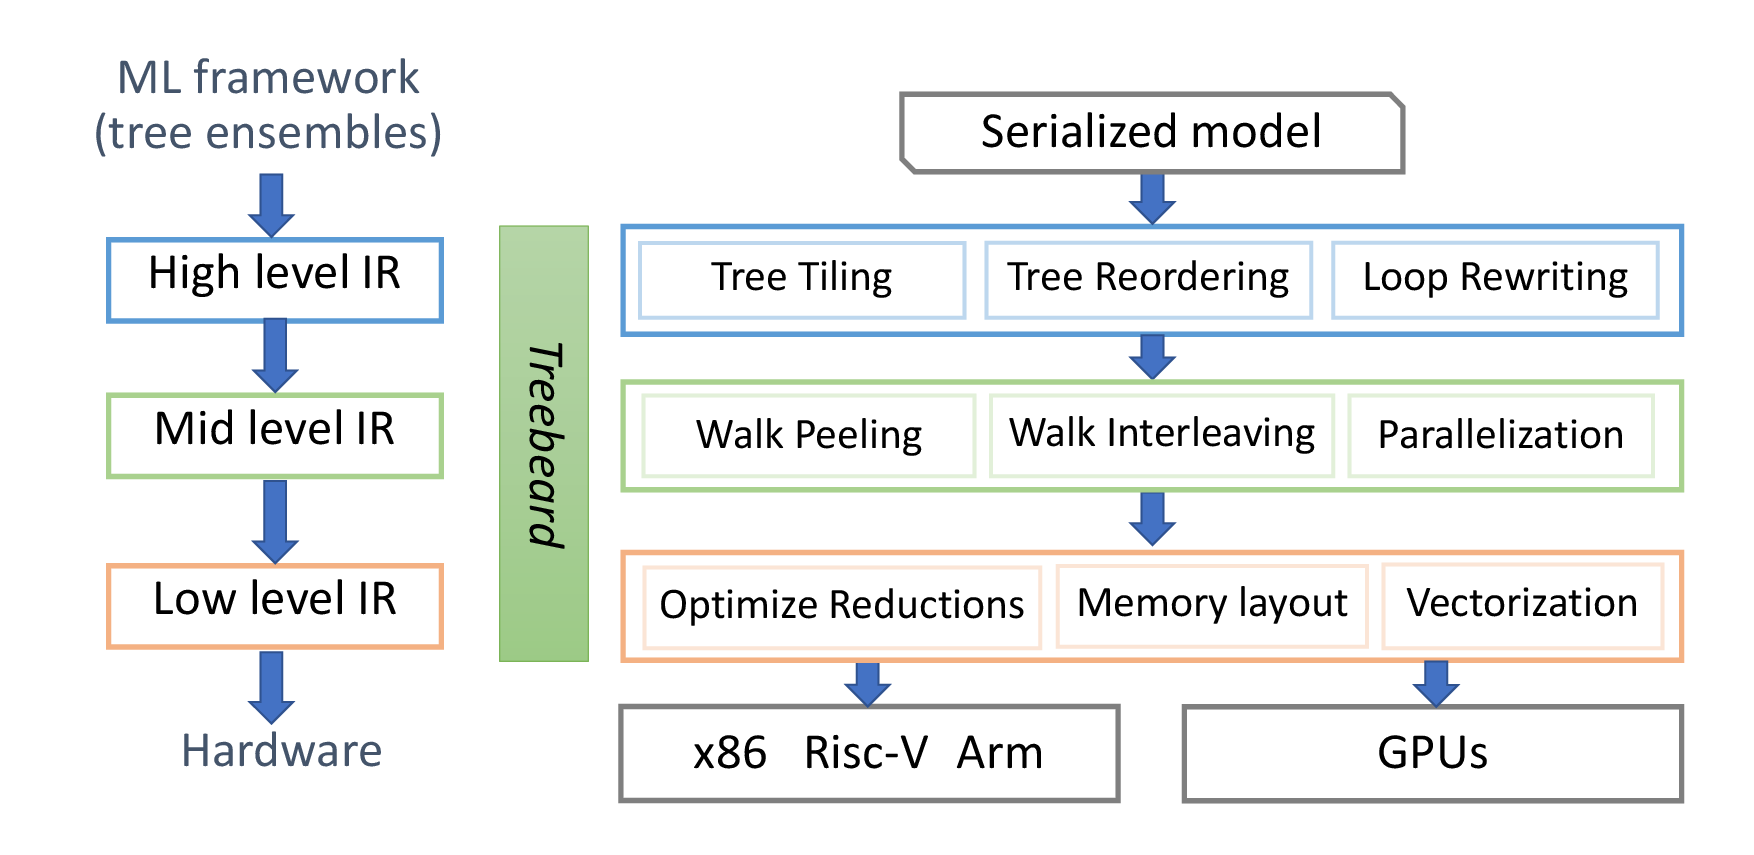
\includegraphics[width=\linewidth]{figures/compiler.png}
  \caption{\Treebeard{} compiler structure.}
  \label{Fig:CompilerStructure}
\end{figure}

% \begin{figure*}[htb]
%   \centering
%   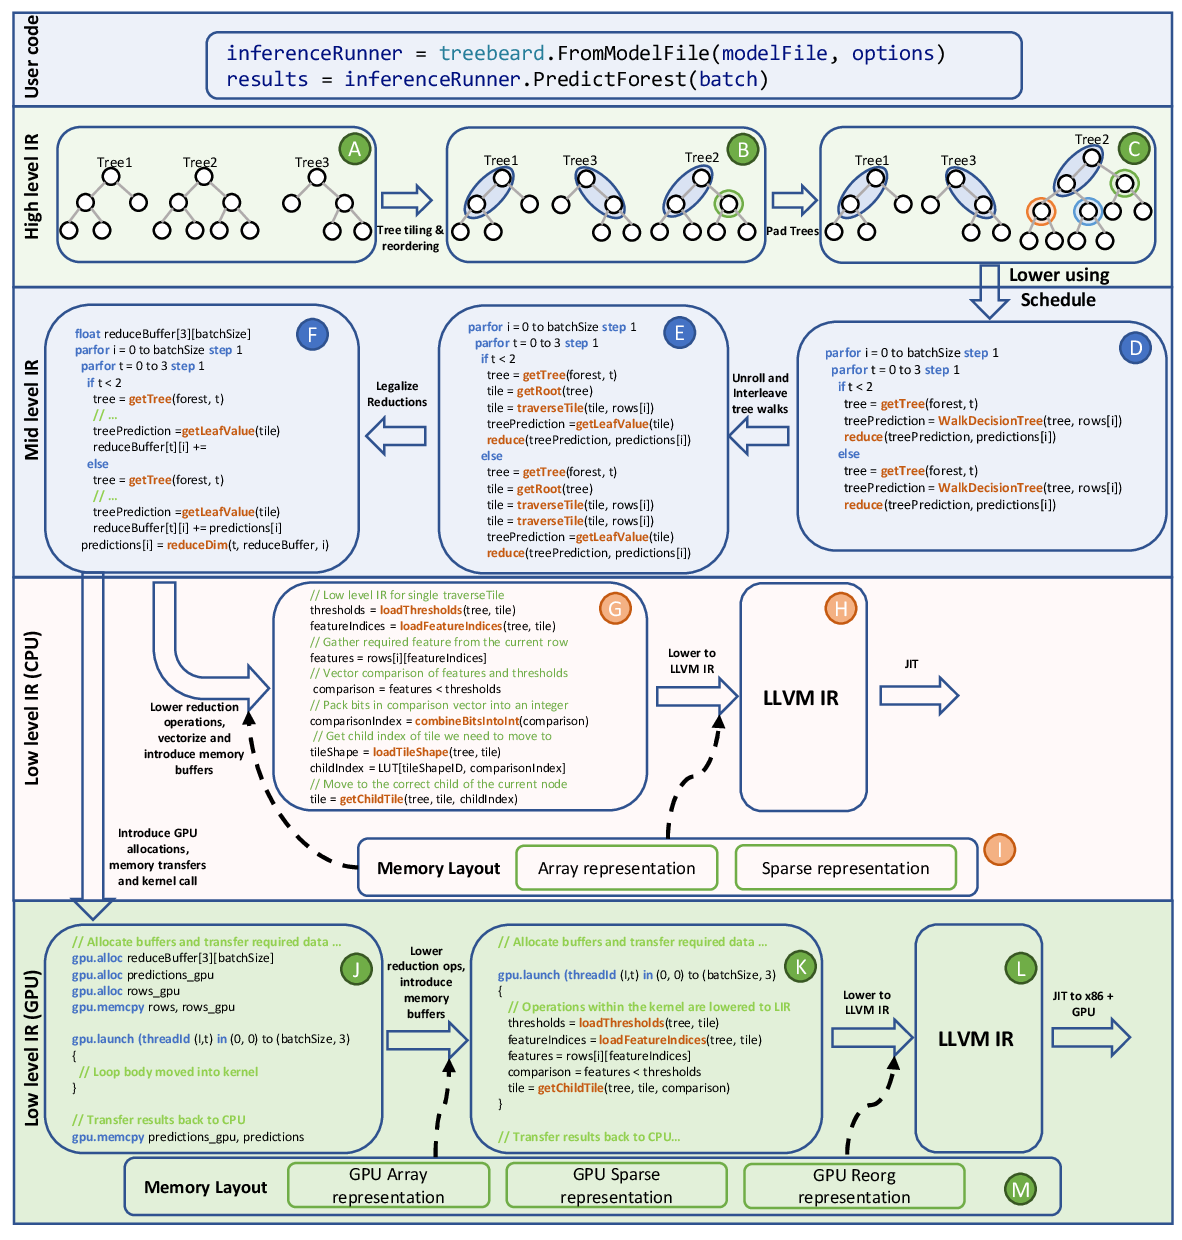
\includegraphics[width=\linewidth]{figures/OverviewExample_New.png}
%   \vskip 10pt
%   \caption{\Treebeard{} IR lowering and optimization details: the three abstraction levels in \Treebeard{}'s IR are shown. The
%            high level IR is a tree-based IR to perform model level optimization, the mid-level IR is for
%            loop optimizations that are independent of memory layout and the low level IR allows us to perform
%            vectorization and other memory layout dependent optimizations.}
%   \label{Fig:LoweringExample}
% \end{figure*}

\begin{figure*}[htb]
  \centering
  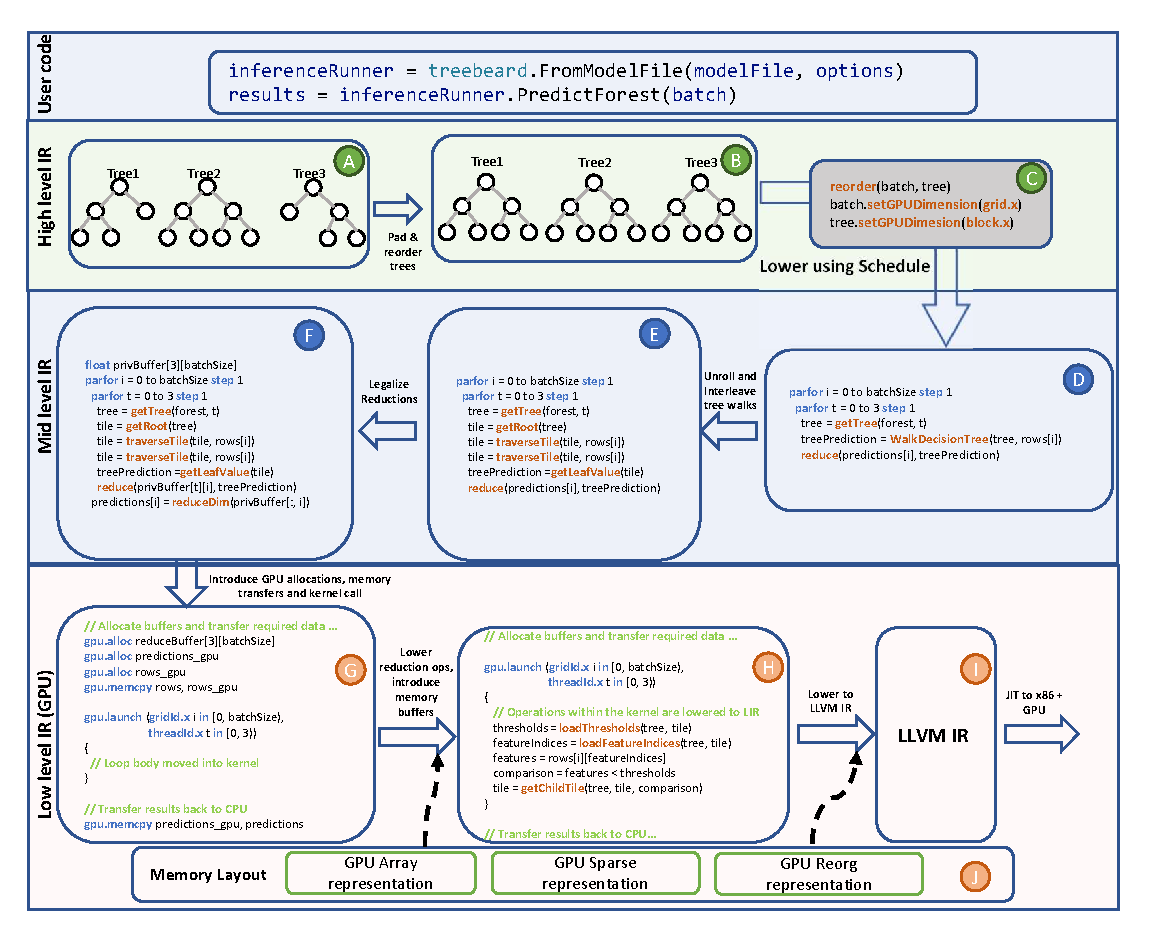
\includegraphics[width=\linewidth]{figures/GPUCompilationOverview-cropped.pdf}
  \vskip 10pt
  \caption{\Treebeard{} IR lowering and optimization details: the three abstraction levels in \Treebeard{}'s IR are shown. The
           high level IR is a tree-based IR to perform model level optimization, the mid-level IR is for
           loop optimizations that are independent of memory layout and the low level IR allows us to perform
           vectorization and other memory layout dependent optimizations.}
  \label{Fig:GPULoweringExample}
\end{figure*}

In HIR, the model is represented as a collection of binary trees. This abstraction
allows the implementation of optimizations that require the manipulation of the model
or its constituent trees. In Figure \ref{Fig:LoweringExample}, \circled{A}
shows this representation for a model with three trees. 
In HIR, \Treebeard{} tiles tree nodes together to convert
the binary tree to an n-ary tree as shown in \circled{B}. Trees are also 
reordered to enable better code generation and padded to allow more 
efficient traversal as shown in \circled{C}. While these are the optimizations currently 
implemented in \Treebeard{}, these are by no means the only ones that 
are enabled by HIR. It is not difficult to imagine optimizations 
such as tree pruning for specified accuracy levels for example.
These optimizations and rewrites that are performed on the domain-specific 
HIR would have been much on a traditional loop based IR or even in 
other IRs within \Treebeard{}.


After these model-level optimizations are performed on the HIR, the 
code is lowered to the mid-level IR (MIR) as dictated by a user specified schedule
(\circled{C} to \bluecircled{D}) in Figure \ref{Fig:LoweringExample}). The schedule specifies how
the iteration space that goes over the trees and input rows is to be traversed. 
It specifies how the iteration space is to be tiled, which loops are to be
parallelized, which loops are to be mapped to GPU grid and block dimensions etc.
(Details in Section \ref{Sec:SchedulingLang}). MIR is a loop-based IR that 
explicitly encodes details of the iteration space has to be traversed. However, 
it still abstracts details about the in-memory representation of the model. 
Optimizations such as tree-walk unrolling and interleaving are performed 
on the MIR (\bluecircled{E}). Subsequently, reduction operations are split and rewritten 
to correctly and explicitly implement reduction in the presence of 
parallel loops (\bluecircled{F}). More details of this process that we call 
\emph{legalization} are in Section \ref{Sec:Reduction}. Another important 
point to note is that MIR is independent of the target processor and therefore
all optimizations on MIR can be reused across CPU and GPU compilation.

The MIR is then further lowered to a low-level IR (LIR). This is the
level at which the compilation pipeline diverges for CPUs and GPUs. In 
the GPU compilation pipeline, the required memory transfers and kernel
invocations are inserted into the LIR (\circled{J}). Additionally, buffers 
to hold model values are inserted and tree operations are lowered to
explicitly refer to these buffers. This lowering is controlled by 
a plugin mechanism where different in-memory representations can 
be added to the compiler by implementing an interface. These plugins
provide information required for the lowering of MIR to LIR as well as 
the lowering to LLVM IR as shown in Figure \ref{Fig:LoweringExample}.
Again, a significant amount of code is shared between the
CPU and GPU pipelines for representations that are common between them
(Array and Sparse representations). Vectorization of tree traversals 
is also explicitly represented in LIR.

To reiterate, the following are the salient points of \Treebeard{}'s design.
\begin{enumerate}
  \item The compiler uses three intermediate representations (IRs) to
  represent the inference computation at different levels of abstraction. This
  allows different optimizations to be performed and also allows us to share
  infrastructure between compilation pipelines for different target processors.

  \item The specification of how the inference computation is to be lowered to 
  loops is not encoded directly in the compiler. Instead, this 
  is specified as an input to the compiler using a scheduling language that is 
  specialized for decision tree inference computations (Section \ref{Sec:SchedulingLang}).
  This separation allows us to build optimizations and schedule exploration 
  mechanisms independent of the core compiler (Section \ref{AutoTuneHeuristic}). 
  The scheduling language also exposes details like parallelization, optimization
  of reductions (vectorization, use atomics, shared memory on GPUs etc.).

  \item \Treebeard{} has been designed to keep the optimization passes and code 
  generator independent of the in-memory representation finally used for the model. To achieve 
  this, \Treebeard{} specifies an interface to implement that provides the necessary 
  capabilities to the code generator as a plugin. This interface abstracts several details
  on how model values are stored. In particular, it abstracts the actual layout of 
  the memory buffers, how to load model values like thresholds and feature indices, how 
  to move from a node to its children and determining whether a node is a leaf.
  This design allows us to write each memory representation as a standalone plugin 
  and reuse the rest of the compiler infrastructure.
\end{enumerate}
\section{Scheduling Language}
\label{sec:schedule}
As we articulated in Section \ref{sec:intro}, there are several 
different configurations and optimizations strategies for decision 
tree inference. The best ones are significantly different across
models, batch sizes and hardware platforms. Therefore, designing
any one hard-coded lowering strategy is not feasible as this would 
make portable performance impossible. To address this problem, we 
design a scheduling language for \Treebeard{}. The scheduling 
language provides an abstract way to specify loop structure and 
other optimizations as an input to the compiler. Making the 
scheduling specification external to the compiler allows to build 
auto-schedulers and auto-tuners (Section \ref{sec:exploring}).
Using a scheduling language will also significantly simplify 
adding support for new hardware as this will likely require
different locality optimizations and loop transformations.

The goal of \Treebeard{}'s scheduling language is to declaratively
express loop structures and the application of other optimizations 
(tree walk unrolling, tree walk interleaving etc.). 

\subsection{Language Definition}
The core construct of \Treebeard{}'s scheduling language is an 
\textbf{\emph{index variable}} which abstractly represents a loop. 
The language then provides directives to manipulate these index 
variables. There are two special index variables -- \op{batch} and
\op{tree} that are used to represent the batch and tree loops and all 
other index variables are derived from these. A schedule derives 
new index variables from these root index variables by applying
directives. 

\Treebeard{}'s scheduling language has three classes of directives. The first is a set 
of loop modifiers that are used to specify the structure of the loop nest to
walk the iteration space (Table \ref{Tab:LoopModifiers}). The second is a set of 
directives that enable optimizations on a loop (Table \ref{Tab:Optimizations}). 
Finally, we have a class of attributes that enable reduction specific optimizations
(Table \ref{Tab:ReductionOpts}).

% \subsubsection{Loop Modifiers}
% The clauses modify these index variables or 
% index variables derived from these (through the application of clauses).
% \begin{itemize}
%   \item \textbf{tile}: Tile the passed index variable using a fixed tile size.
%   \item \textbf{split}: Split the range of the passed index variable into two parts. The range of the first part is specified
%   by an argument.
%   % \item \textbf{unroll}: Unroll an index completely
%   \item \textbf{reorder}: Reorder the specified indices. The specified indices must be successive indices in the current loop nest.
%   \item \textbf{specialize}: Generate separate code for each iteration of the specified index variable. This is useful 
%   while parallelizing across trees and these trees have different depths.
%   \item \textbf{gpuDimension}: Maps the specified index variable to represent a dimension in either the GPU kernel grid or thread block.
% \end{itemize}

\begin{table}[htb]
  \centering
  \resizebox{\linewidth}{!}{
  \begin{tabularx}{\linewidth}{c | l | l}
   \toprule
   \textbf{Directive} & \textbf{Inputs} & \textbf{Description} \\
   \midrule
   \multirow{4}{*}{\texttt{tile}} & \textbf{indexVar}  & \multirow{4}{*}{\parbox{0.55\linewidth}{Tile the loop corresponding to \textbf{indexVar}
   with the specified tile size. Resulting loops will be represented by \textbf{outer} and \textbf{inner}.}} \\
                                               &  \textbf{outer} & \\
                                               &  \textbf{inner} &  \\
                                               &  \textbf{tileSize} &  \\
   \midrule
   \multirow{6}{*}{\texttt{split}} & \textbf{indexVar}  & \multirow{6}{*}{\parbox{0.55\linewidth}{Fiss the loop represented by \textbf{indexVar}
   at iteration \textbf{splitIter}. Resulting loops will be represented by \textbf{first} and \textbf{second}. Returns a maps from nested 
   index variables to new ones created by splitting.}} \\
                                               &  \textbf{first} & \\
                                               &  \textbf{second} &  \\
                                               &  \textbf{splitIter} &  \\
                                               & & \\
                                               & & \\

   \midrule
   \multirow{4}{*}{\texttt{reorder}} & \textbf{indices[]}  & \multirow{4}{*}{\parbox{0.55\linewidth}{Permute loops corresponding to the specified index variables.
   The loops must be perfectly nested in the current loop structure.}} \\
                                               &   & \\
                                               &   &  \\
                                               &   &  \\
   \midrule
   \multirow{4}{*}{\texttt{specialize}} & \textbf{indexVar}  & \multirow{4}{*}{\parbox{0.55\linewidth}{Generate specialized code for each iteration of the loop. 
   Useful when different iterations of a loop need to execute different code.}} \\
                                               &   & \\
                                               &   &  \\
                                               &   &  \\
   \midrule
   \multirow{3}{*}{\texttt{gpuDimension}} & \textbf{indexVar}  & \multirow{3}{*}{\parbox{0.55\linewidth}{Map the passed index variable to a dimension of either the grid
   or thread block.}} \\
                                               & \textbf{gpuDim}  & \\
                                               &   &  \\

  \bottomrule
  \end{tabularx}
  }
  \vskip 5pt
  \caption{\label{Tab:LoopModifiers} List of all the loop modifiers in \Treebeard{}'s scheduling language. We use \emph{index variable}
  and \emph{loop} interchangeably in descriptions for clarity of exposition.}
\end{table}


% The following are examples of how the loop modifiers can be used.
% \begin{itemize}
%   \item The loop order used by XGBoost\cite{XGBoost} is (tree, batch) -- walk one tree for all inputs in the batch before 
%   moving to the next tree. The corresponding schedule would be
% \begin{lstlisting}[style=c++]
%   reorder(tree, batch)
% \end{lstlisting}

%   \item The below schedule computes 2 trees at a time over the whole batch.
% \begin{lstlisting}[style=c++]
%   tile(tree, t0, t1, 2)
%   reorder(t0, batch, t1)
% \end{lstlisting}

%   \item If we additionally only want to compute over 4 input rows (rather than the whole batch) for
%   every 2 tree, and then move onto the next 2 trees for the same set of inputs, then the schedule is as follows. 
% \begin{lstlisting}[style=c++]
%   tile(batch, b0, b1, 4) 
%   tile(tree, t0, t1, 2)
%   reorder(b0, t0, b1, t1) 
% \end{lstlisting}

% \end{itemize}

% \subsubsection{Optimizations}
% The following clauses provide ways to optimize the inference routine being generated.
% \begin{itemize}
%   \item \textbf{cache}: Cache the working set of one iteration of the specified loop corresponding
%   to this index. This can be specified on either batch or tree loops. Specifying it 
%   on a batch loop leads to all rows accessed in a single iteration of the loop 
%   being cached. Similarly, specifying it on a tree loop leads to all trees accessed in 
%   one iteration of that loop being cached.
%   \item \textbf{parallel}: Execute the loop corresponding to this index in parallel.
%   \item \textbf{interleave}: Interleave the execution of the tree walks within the current index (must be applied on an inner most index).
%   \item \textbf{unrollWalk}: Unroll tree walks at the current index. 
%   \item \textbf{peelWalk}: Peel the first n steps of the specified tree walk and don't check for leaves for that number of steps.
% \end{itemize}

\begin{table}[htb]
  \centering
  \resizebox{\linewidth}{!}{
  \begin{tabularx}{\linewidth}{c | l | l}
   \toprule
   \textbf{Directive} & \textbf{Inputs} & \textbf{Description} \\
   \midrule
   \multirow{4}{*}{\texttt{cache}} & \textbf{indexVar}  & \multirow{4}{*}{\parbox{0.55\linewidth}{Cache the working set of one iteration of the specified loop. 
   Cache rows for a batch loop and trees for a tree loop.}} \\
                                               &  &  \\
                                               &  &  \\
                                               &  &  \\
   \midrule
   \multirow{2}{*}{\texttt{parallel}} & \textbf{indexVar}  & \multirow{2}{*}{\parbox{0.55\linewidth}{Execute the iterations of the specified 
   loop in parallel.}} \\
                                               &  & \\

   \midrule                                               
   \multirow{3}{*}{\texttt{interleave}} & \textbf{indexVar}  & \multirow{3}{*}{\parbox{0.55\linewidth}{Interleave tree walks within the specified 
   loop (must be innermost loop).}} \\
                                               &  & \\
                                               &  & \\

   \midrule                                               
   \multirow{3}{*}{\texttt{unrollWalk}} & \textbf{indexVar}  & \multirow{3}{*}{\parbox{0.55\linewidth}{Unroll tree walks at the specified loop 
   for \textbf{unrollDepth} hops. Loop must be an innermost loop.}} \\
                                               & \textbf{unrollDepth} & \\
                                               &  & \\

  \bottomrule
  \end{tabularx}
  }
  \vskip 5pt
  \caption{\label{Tab:Optimizations} List of optimization directives in \Treebeard{}'s scheduling language. 
  We use \emph{index variable} and \emph{loop} interchangeably in descriptions for clarity of exposition.}
\end{table}


% \subsubsection{Reduction Optimization}
% \begin{itemize}
%   \item \textbf{atomicReduce}: Use atomic memory operations to accumulate values across 
%   parallel iterations of the specified loop. 
%   \item \textbf{sharedReduce}: Only applies to GPU compilation. Specifies that intermediate
%   results are to be stored in shared memory.
%   \item \textbf{vectorReduce}: Use vector instructions with the specified vector width 
%   to reduce intermediate values across parallel iterations of the specified loop.
% \end{itemize}

\begin{table}[htb]
  \centering
  \resizebox{\linewidth}{!}{
  \begin{tabularx}{\linewidth}{c | l | l}
   \toprule
   \textbf{Directive} & \textbf{Inputs} & \textbf{Description} \\
   \midrule
   \multirow{3}{*}{\texttt{atomicReduce}} & \textbf{indexVar}  & \multirow{3}{*}{\parbox{0.55\linewidth}{Use atomic memory operations to accumulate values across 
   parallel iterations of the specified loop.}} \\
                                               &  &  \\
                                               &  &  \\
   \midrule
   \multirow{3}{*}{\texttt{sharedReduce}} & \textbf{indexVar}  & \multirow{3}{*}{\parbox{0.55\linewidth}{Specifies that intermediate
   results are to be stored in shared memory (GPU only).}} \\
                                               &  & \\
                                               &  & \\

   \midrule                                               
   \multirow{4}{*}{\texttt{vectorReduce}} & \textbf{indexVar}  & \multirow{4}{*}{\parbox{0.55\linewidth}{Use vector instructions with the specified vector width 
   to reduce intermediate values across parallel iterations of the specified loop.}} \\
                                               & \textbf{width} & \\
                                               &  & \\
                                               &  & \\

  \bottomrule
  \end{tabularx}
  }
  \vskip 5pt
  \caption{\label{Tab:ReductionOpts} List of reduction optimization directives in \Treebeard{}'s scheduling language. 
  We use \emph{index variable} and \emph{loop} interchangeably in descriptions for clarity of exposition.}
\end{table}


%\TODO{Add examples for RAPIDS, Tahoe (Maybe show some strategies can be encoded?)}

We now show how the implementation strategies of several existing systems can 
be encoded in \Treebeard{}'s scheduling language. First, we note that the 
default loop order is [\op{batch}, \op{tree}], i.e, for each row in the input
batch, go over all trees.

% \subsection{The XBoost Schedule}
XGBoost\cite{XGBoost} implements inference on the CPU by going 
over a fixed number of rows (64 in the previous version)
for every tree and then moving to the next tree. When all trees 
have been walked for this set of rows, the next set of rows is 
taken up. Also, different sets of rows are processed in parallel.
This schedule can be implemented in \Treebeard{}'s scheduling language 
as follows.
\begin{lstlisting}[style=c++]
  tile(batch, b0, b1, CHUNK_SIZE)
  reorder(b0, tree, b1)
  parallel(b0)
\end{lstlisting}

Tahoe\cite{Tahoe} has four strategies for inference on the GPU that it picks from for a given model. 
We show how two of these strategies can be encoded using \Treebeard{}'s scheduling language.
The rest can be encoded similarly. 
\begin{itemize}
  \item \textbf{Direct Method}: In this strategy, a single GPU thread walks all trees
  for a given input row. The schedule for this strategy is as follows.
\begin{lstlisting}[style=c++]
  tile(batch, b0, b1, ROWS_PER_TB)
  reorder(b0, b1, tree)
  gpuDimension(b0, grid.x)
  gpuDimension(b1, block.x)
\end{lstlisting}
  Here, \op{ROWS\_PER\_TB} is the number of rows that are processed by a single thread block.
  \item \textbf{Shared Data}: In this strategy, a thread block walks all the trees 
  for a given row in parallel. If threads walk multiple trees, each thread accumulates
  partial results. Finally, a thread block wide reduction is performed to compute 
  the prediction. The schedule for this strategy is as follows.
\begin{lstlisting}[style=c++]
  reorder(batch, tree)
  gpuDimension(batch, grid.x)
  gpuDimension(tree, block.x)
  cache(batch)
\end{lstlisting}
%   \item \textbf{Shared Forest}: In this strategy, the whole model is loaded into 
%   shared memory and subsequently, a single thread walks all trees for a particular
%   row. The schedule for this strategy is as follows.
% \begin{lstlisting}[style=c++]
%   tile(batch, b0, b1, ROWS_PER_TB)
%   tile(tree, t0, t1, N_TREES)
%   reorder(b0, b1, t0, t1)
%   cache(t0)
%   gpuDimension(b0, grid.x)
%   gpuDimension(b1, block.x)
% \end{lstlisting}
%   Here, we create a placeholder single iteration loop \op{t0} so that we can 
%   specify that all trees are to be cached.
%   \item \textbf{Shared Partial Forest}: In case the model is too large to fit into
%   shared memory, the model is split into chunks and each chunk is loaded into shared
%   memory. Again, as in the previous strategy, one thread walks all trees assigned to
%   a thread block for a row. The schedule for this strategy is as follows.
% \begin{lstlisting}[style=c++]
%   tile(batch, b0, b1, ROWS_PER_TB)
  
%   tile(tree, t0, t0Inner, TREES_PER_TB)
%   tile(t0Inner, t1, t2, TREES_PER_TB)
%   cache(t1)
%   reorder(b0, t0, b1, t1, t2)

%   gpuDimension(b0, grid.x)
%   gpuDimension(t0, grid.y)
%   gpuDimension(b1, block.x)
% \end{lstlisting}
\end{itemize}

There are some simplifying assumptions and limitations in the current design
of the scheduling language. Mainly, tree traversals are considered atomic and
accumulation of tree predictions is done immediately (as opposed to, 
for example, collecting all predictions and performing a reduction later).
However, we find that these are not significant limitations in practice as
the current design is able to express most strategies of interest.
\section{Representing and Optimizing Reductions}
\label{sec:reduction}
\Treebeard{} needs to sum up individual tree predictions to compute 
the prediction of the model while performing inference. However,
generating fused reductions within arbitrary loop nests specified 
using \Treebeard{}'s scheduling language is non-trivial. We found 
that existing reduction support in MLIR is insufficient to code
generate and optimize these reductions. MLIR only supports reductions
of value types and does not provide ways to lower reductions to GPUs. 
To address this gap, we design an MLIR dialect that allows us to
specify accumulating values into an element of a multi-dimensional array
and can be lowered to CPU or GPU. 

The main abstraction we introduce is the \op{reduce} op. It models 
atomically accumulating values into an element of a 
multi-dimensional array (represented by an MLIR \op{memref}).
Consider the following \Treebeard{} schedule.
In our example, \op{N\_t} is the number of trees 
and \op{batch\_size} is the batch size. The schedule tiles the 
tree loop and parallelizes the resulting outer loop.
\begin{lstlisting}[style=c++]
  tile(tree, t0, t1, N_t/2);
  reorder(t0, t1, batch);
  parallel(t0);
\end{lstlisting}

The MIR generated by \Treebeard{} for the above schedule is as follows. 
\begin{lstlisting}[style=c++]
  float result[batch_size]
  model = ensemble(...) 
  par.for t0 = 0 to N_t step N_t/2:
    for t1 = 0 to N_t/2:
      for batch = 0 to batch_size:
        t = getTree(model, t0 + t1) 
        p = walkDecisionTree(t, rows[batch])
        reduce(result[batch], p)
\end{lstlisting}

The compiler simply generates a \op{reduce} op to perform
the required parallel reduction. 
The semantics of the \op{reduce} op is exactly the semantics of 
an atomic accumulation, i.e. it guarantees that all accumulations 
are correctly performed even in the presence of parallel loops. 
The \op{reduce} op is defined for all associative and commutative
reduction operations with a well-defined initial value. The 
reduction operator and the initial value are attributes applied
on the \op{reduce} op. 

Having modeled the reductions with an abstract operation, the 
aim now is to lower this to a correct and optimized 
implementation on both CPU and GPU. In order to do this, we 
first determine if any parallel loop iterations can accumulate 
into the same array element. We call such loops 
\emph{\textbf{reduction loops}}. If such loops exist, we 
\textbf{\emph{privatize}} the array for each iteration of the
loop. We call this process \textbf{\emph{legalization}}.
Subsequently, each privatized dimension 
can be reduced at the end of the reduction loop it was inserted for. 
%\TODO{We cannot do better than this in terms of memory usage} \TODO{Need a proof}.

In our example, \Treebeard{} determines that the \op{t0} loop is a reduction 
loop w.r.t the \op{result} array and therefore legalizes 
the reduction by inserting a privatized array 
\op{partResults}. The privatized dimension of this array 
is reduced at the end of the \op{t0} loop.

\begin{lstlisting}[style=c++]
  float result[batch_size], partResults[2][batch_size]
  model = ensemble(...) 
  par.for t0 = 0 to N_t step N_t/2:
    for t1 = 0 to N_t/2:
      for batch = 0 to batch_size:
        t = getTree(model, t0 + t1) 
        p = walkDecisionTree(t, rows[batch])
        reduce(partResults[t0/(N_t/2)][batch], p)
  
  results = reduceDimension(partResults[:, :], 0)
\end{lstlisting}

The op \op{reduceDimension} reduces values across the specified
dimension of an n-dimensional array. Here, 
it reduces all elements of the first dimension (dimension 0). 
and produces a result memref with a single dimension of size \op{batch\_size}.

To reduce the amount of memory used by arrays introduced for reduction,
we introduce the \op{reduceDimInplace} operation. It is similar to the 
\op{reduceDimension} op except that it updates the input array inplace
rather than writing results to a target array. It writes results to the 
zeroth index of the dimension being reduced. We use this op to 
compute intermediate results when several reduction loops are identified.

% \begin{definition}
%  \textbf{\op{reduce\_dimension\_inplace(memref, dim, [indices], [rangeStart], [rangeEnd])}}:
%   Computes the reduction over the dimension specified by \op{dimension} and stores the 
%   result at index 0 of that dimension. \op{[indices]} must be a vector of \op{dim} elements
%    (or empty if the dimension being reduced is the first dimension). \op{[rangeStart]} 
%    and \op{[rangeEnd]} must have the same number of elements. If both are \op{null} (not passed), 
%    all elements of the corresponding dimension are reduced. 
  
%   The computation performed by the op is defined by the following equation.
  
%   $memref[\vec{\boldsymbol{indices}}, 0, \vec{\boldsymbol{k}}] = \sum_{i=0}^{shape[dim]} memref[\vec{\boldsymbol{indices}}, i, \vec{\boldsymbol{k}}]\quad   \forall \vec{\boldsymbol{k}} \in \left[[rangeStart_0, rangeEnd_0), ... , [rangeStart_n, rangeEnd_n)\right]$  
% \end{definition}

\subsection{Lowering Reduction Operations}
% We implement lowering of the operations defined above to both the CPU and GPU.
% Since the lowering pipeline from MIR to LIR are different for CPU and GPU 
% compilation, we implement lowering and optimization of our reduction dialect to CPUs and
% GPUs simply using different MLIR rewrite patterns. 
In this section, we briefly describe 
how we lower the reduction operations to the CPU and GPU. 

For both CPU and GPU, \op{reduce} is lowered to a sequence 
of load, compute and write operations. This is possible because 
legalization ensures that parallel threads do not write to the same 
array element. 
%\subsubsection{Lowering to CPU}

For CPUs, we lower \op{reduceDimInplace} and 
\op{reduceDimension} to a simple loop nest that goes over the specified
subset of the input array, performs the reduction and writes 
the result into the appropriate location of the target array. 
If the schedule specifies that the reduction is to be vectorized,
the lowering passes generate vector (LLVM IR) instructions for 
the reduction.
% then as many elements as specified by the vector width are read 
% from the input array as a vector, accumulated as a vector, and 
% finally written back to the target array.

% In general, this works 
% well because reductions are typically being performed on dimensions
% other than the inner-most dimension and therefore, this strategy
% loads successive elements from memory maximizing memory bandwidth 
% utilization. 

% \TODO{explain atomic reduction}

% \subsubsection{Lowering to GPU}
The same reduction abstractions can be lowered to efficient GPU implementations
and therefore, simplify higher-level code generation. 
% The lowering for 
% the inplace and non-inplace operations are essentially the same, except 
% for the target array and we do not distinguish between them except 
% for finally storing the result. 
%
% The lowering of the \op{reduceDim*} 
\Treebeard{} can lower these ops to either exploit
parallelism across the independent reductions or 
the inherent parallelism in the reduction by performing a divide and conquer 
reduction depending on whether there are enough independent reductions to keep all threads
in a thread block busy.
% then the lowering pass can generate code that performs one (or 
% multiple) reductions in each thread. If, however, there are not 
% enough independent reductions, then the lowering pass generates a tree 
% style reduction where multiple threads cooperate to perform a single reduction
% using inter-thread shuffles.

% Another feature specific to GPU reductions is the use of shared memory. 
Additionally, if the schedule specifies that the reduction needs to be performed 
using shared memory, the privatized buffer is allocated in shared memory. 
% The compiler only allocates as much shared memory 
% as needed to hold values processed by a single thread-block.
%  and 
% index offsets are appropriately rewritten to handle the differences between 
% the indexing of the target memref and the shared memory array.
Our abstractions for reductions allow our lowering passes to be 
agnostic of whether we use shared memory and therefore allow 
us to enable or disable shared memory use independently from the other 
parts of the compiler. 

% We find that our current implementation of lowering reduction operations 
% is sufficient for \Treebeard{} and reduction is not the bottleneck in the
% generated code. However, we believe this approach to enabling 
% higher level code generators to easily generate reductions 
% through simple abstractions and then having the compiler 
% automatically lower them to efficient implementation is an
% important area for future work with applicability in several 
% domains. 

%\TODO{Should we mention how we handle multi-class models?}

\section{Citations and Bibliographies}

Artifacts:
  \cite{MLIR} and \cite{LLVM}.


%%
%% The next two lines define the bibliography style to be used, and
%% the bibliography file.
\bibliographystyle{ACM-Reference-Format}
\bibliography{refs}

%%
%% If your work has an appendix, this is the place to put it.

\end{document}
\endinput
%%
%% End of file `sample-sigplan.tex'.
